\documentclass{exam}

\usepackage{units} 
\usepackage{graphicx}
\usepackage[fleqn]{amsmath}
\usepackage{cancel}
\usepackage{float}
\usepackage{mdwlist}
\usepackage{booktabs}
\usepackage{cancel}
\usepackage{polynom}
\usepackage{caption}
\usepackage{fullpage}
\usepackage{comment}
\usepackage{enumerate}
\usepackage{xfrac}

\newcommand{\degree}{\ensuremath{^\circ}} 
\everymath{\displaystyle}

% \begin{figure}[H]
%   \centering
%   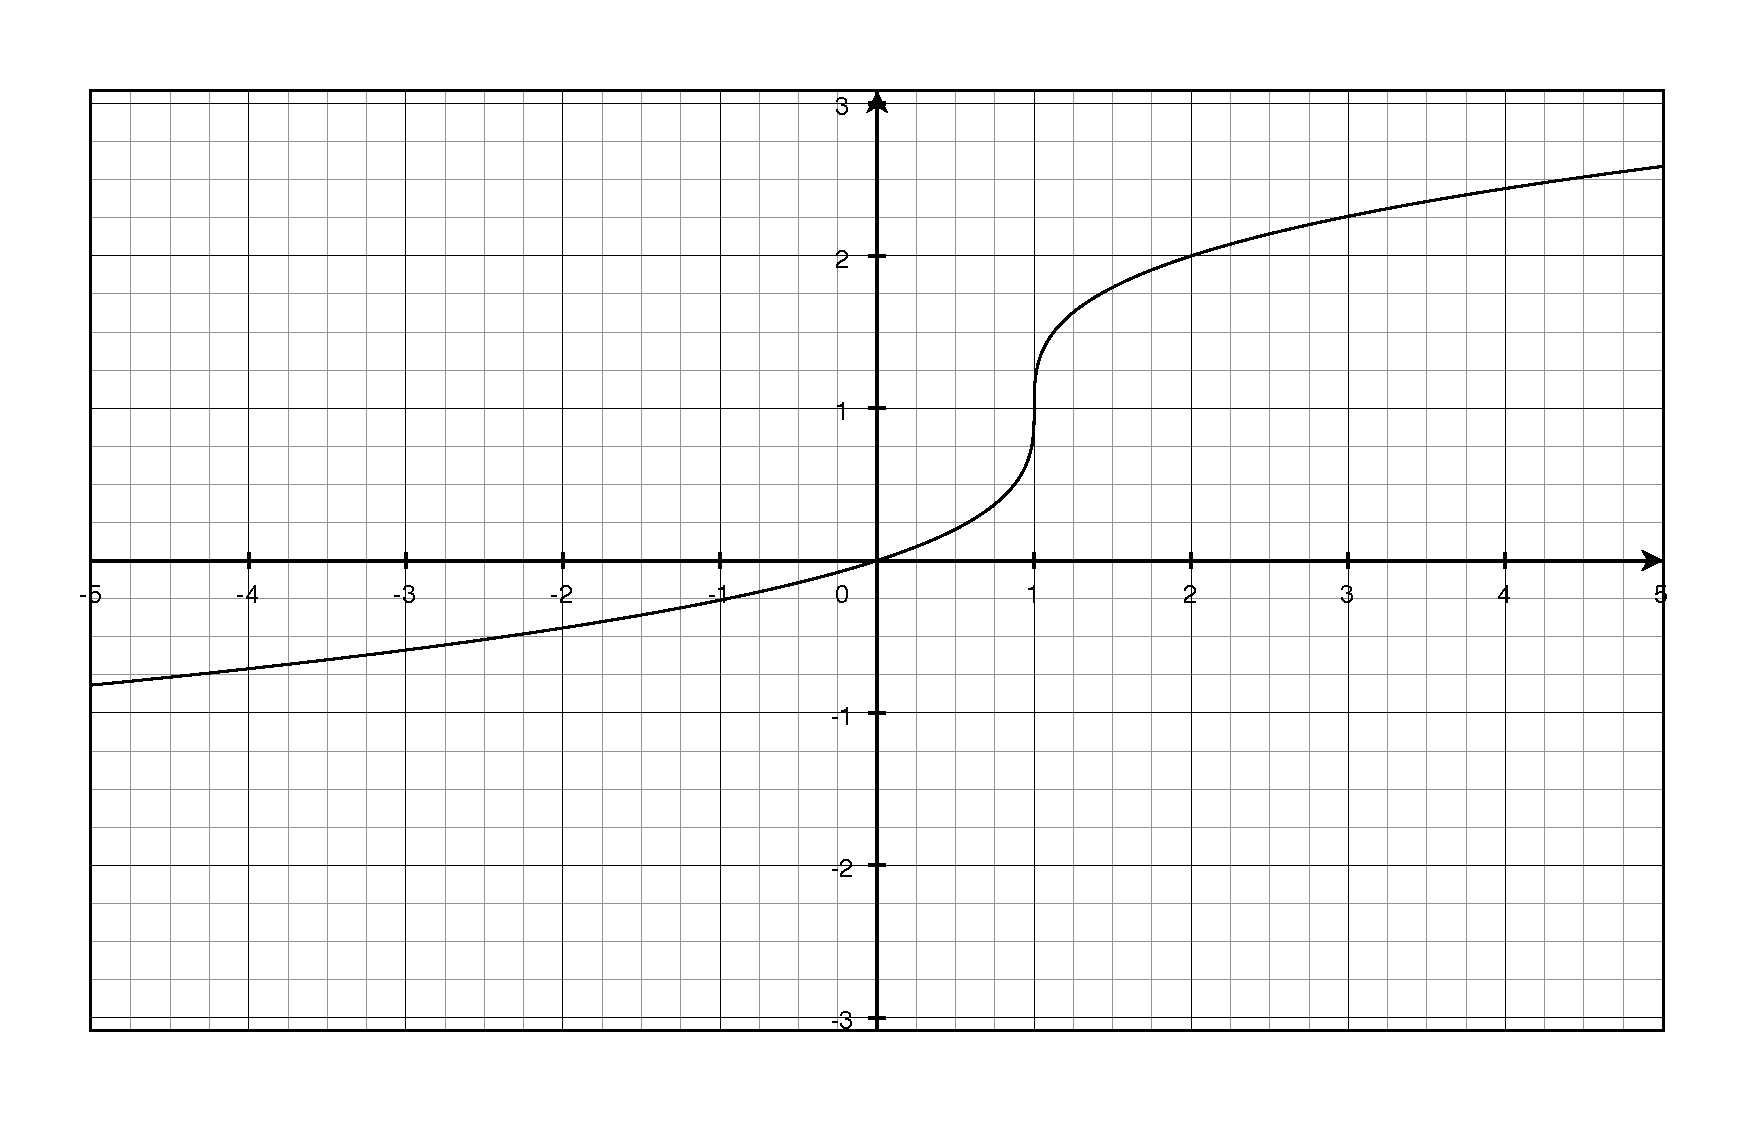
\includegraphics[scale=.3]{question7.eps}
%   \caption*{question 7}
% \end{figure}

% \begin{tabular}{cc}
%   \toprule
%   period & amplitude \\
%     $\pi$ & $2$ \\
%   \bottomrule
% \end{tabular}

\printanswers
\excludecomment{comment}

\ifprintanswers 
  \usepackage{2in1, lscape} 
\fi

\author{}
\date{September 11, 2013}
\title{Math 142 \\ Homework Three}

\begin{document}

  \maketitle

  \section{Homework}
  Section 5.3: 1-5, 12-18, 23-48, 75-76

  \section{Extra Credit}
  Section 5.3: 82

  \ifprintanswers

    \section{Section 5.3}
    \begin{description}

      \item[1]
        \begin{figure}[H]
          \centering
          \includegraphics[scale=0.8]{exercise01.eps}

          $f(x) = 1 + \cos x$
        \end{figure}

      \item[2]
        \begin{figure}[H]
          \centering
          \includegraphics[scale=0.8]{exercise02.eps}

          $f(x) = 3 + \sin x$
        \end{figure}

      \item[3]
        \begin{figure}[H]
          \centering
          \includegraphics[scale=0.8]{exercise03.eps}

          $f(x) = -\sin x$
        \end{figure}

      \item[4]
        \begin{figure}[H]
          \centering
          \includegraphics[scale=0.8]{exercise04.eps}

          $f(x) = 2 - \cos x$
        \end{figure}

      \item[5]
        \begin{figure}[H]
          \centering
          \includegraphics[scale=0.8]{exercise05.eps}

          $f(x) = -2 + \sin x$
        \end{figure}

      \item[12]
        \begin{figure}[H]
          \centering
          \includegraphics[scale=0.9]{exercise12.eps}

          $g(x) = 4 - 2 \sin x$
        \end{figure}

      \item[13]
        \begin{figure}[H]
          \centering
          \includegraphics[scale=0.9]{exercise13.eps}

          $h(x) = | \cos x |$
        \end{figure}

      \item[14]
        \begin{figure}[H]
          \centering
          \includegraphics[scale=0.9]{exercise14.eps}

          $h(x) = | \sin x |$
        \end{figure}

      \item[15]
        \begin{figure}[H]
          \centering
          \includegraphics[scale=0.8]{exercise15.eps}

          $y = \cos 2x$
        \end{figure}

        \begin{tabular}[H]{lr}
          \toprule
          amplitude & 1 \\
          period    & $\pi$ \\
          \bottomrule
        \end{tabular}

      \item[16]
        \begin{figure}[H]
          \centering
          \includegraphics[scale=0.9]{exercise16.eps}

          $y = - \sin 2x$
        \end{figure}

        \begin{tabular}[H]{lr}
          \toprule
          amplitude & $-1$ \\
          period    & $\pi$ \\
          \bottomrule
        \end{tabular}

      \item[17]
        \begin{figure}[H]
          \centering
          \includegraphics[scale=0.9]{exercise17.eps}

          $y = - 3 \sin 3x$
        \end{figure}

        \begin{tabular}[H]{lr}
          \toprule
          amplitude & $-3$ \\
          period    & $\sfrac{2 \pi}{3}$ \\
          \bottomrule
        \end{tabular}

      \item[18]
        \begin{figure}[H]
          \centering
          \includegraphics[scale=0.9]{exercise18.eps}

          $y = \frac{1}{2} \cos 4x$
        \end{figure}

        \begin{tabular}[H]{lr}
          \toprule
          amplitude & $\sfrac{1}{2}$ \\
          period    & $\sfrac{\pi}{4}$ \\
          \bottomrule
        \end{tabular}

      \item[23]
        \begin{figure}[H]
          \centering
          \includegraphics[scale=0.9]{exercise23.eps}

          $y = -2 \sin 2 \pi x$
        \end{figure}

        \begin{tabular}[H]{lr}
          \toprule
          amplitude & $-2$ \\
          period    & $1$ \\
          \bottomrule
        \end{tabular}

      \item[24]
        \begin{figure}[H]
          \centering
          \includegraphics[scale=0.9]{exercise24.eps}

          $y = -3 \sin \pi x$
        \end{figure}

        \begin{tabular}[H]{lr}
          \toprule
          amplitude & $-3$ \\
          period    & $2$ \\
          \bottomrule
        \end{tabular}

      \item[25]
        \begin{figure}[H]
          \centering
          \includegraphics[scale=0.9]{exercise25.eps}

          $y = 1 + \frac{1}{2} \cos \pi x$
        \end{figure}

        \begin{tabular}[H]{lr}
          \toprule
          amplitude & $\sfrac{1}{2}$ \\
          period    & $2$ \\
          \bottomrule
        \end{tabular}

      \item[26]
        \begin{figure}[H]
          \centering
          \includegraphics[scale=0.9]{exercise26.eps}

          $y = -2 + \cos 4 \pi x$
        \end{figure}

        \begin{tabular}[H]{lr}
          \toprule
          amplitude & $1$ \\
          period    & $\sfrac{1}{2}$ \\
          \bottomrule
        \end{tabular}

      \item[27]
        \begin{figure}[H]
          \centering
          \includegraphics[scale=0.8]{exercise27.eps}

          $y = \cos \left( x - \frac{\pi}{2} \right)$
        \end{figure}

        \begin{tabular}[H]{lr}
          \toprule
          amplitude   & $1$ \\
          period      & $2 \pi$ \\
          phase shift & $\sfrac{\pi}{2}$ \\
          \bottomrule
        \end{tabular}

      \item[28]
        \begin{figure}[H]
          \centering
          \includegraphics[scale=0.8]{exercise28.eps}

          $y = 2 \sin \left( x - \frac{\pi}{3} \right)$
        \end{figure}

        \begin{tabular}[H]{lr}
          \toprule
          amplitude   & $2$ \\
          period      & $2 \pi$ \\
          phase shift & $\sfrac{\pi}{3}$ \\
          \bottomrule
        \end{tabular}

      \item[29]
        \begin{figure}[H]
          \centering
          \includegraphics[scale=0.8]{exercise29.eps}

          $y = - 2 \sin \left( x - \frac{\pi}{6} \right)$
        \end{figure}

        \begin{tabular}[H]{lr}
          \toprule
          amplitude   & $-2$ \\
          period      & $2 \pi$ \\
          phase shift & $\sfrac{\pi}{6}$ \\
          \bottomrule
        \end{tabular}

      \item[30]
        \begin{figure}[H]
          \centering
          \includegraphics[scale=0.8]{exercise30.eps}

          $y = 3 \cos \left( x + \frac{\pi}{4} \right)$
        \end{figure}

        \begin{tabular}[H]{lr}
          \toprule
          amplitude   & $3$ \\
          period      & $2 \pi$ \\
          phase shift & $\sfrac{\pi}{4}$ \\
          \bottomrule
        \end{tabular}

      \item[31]
        \begin{figure}[H]
          \centering
          \includegraphics[scale=0.8]{exercise31.eps}

          $y = -4 \sin 2 \left( x + \frac{\pi}{2} \right)$
        \end{figure}

        \begin{tabular}[H]{lr}
          \toprule
          amplitude   & $-4$ \\
          period      & $\pi$ \\
          phase shift & $\pi$ \\
          \bottomrule
        \end{tabular}

      \item[32]
        \begin{figure}[H]
          \centering
          \includegraphics[scale=0.8]{exercise32.eps}

          $y = \sin \sfrac{1}{2} \left( x + \frac{\pi}{4} \right)$
        \end{figure}

        \begin{tabular}[H]{lr}
          \toprule
          amplitude   & $\sfrac{1}{2}$ \\
          period      & $4 \pi$ \\
          phase shift & $- \sfrac{\pi}{4}$ \\
          \bottomrule
        \end{tabular}

      \item[33]
        \[
          y = 5 \cos \left( 3x - \frac{\pi}{4} \right) = 5 \cos 3 \left( x - \frac{\pi}{12} \right)
        \]

        \begin{figure}[H]
          \centering
          \includegraphics[scale=0.8]{exercise33.eps}

          $y = 5 \cos \left( 3x - \frac{\pi}{4} \right)$
        \end{figure}

        \begin{tabular}[H]{lr}
          \toprule
          amplitude   & $5$ \\
          period      & $\sfrac{2 \pi}{3}$ \\
          phase shift & $\sfrac{\pi}{12}$ \\
          \bottomrule
        \end{tabular}

      \pagebreak

      \item[34]
        \[
          y = 2 \sin \left( \frac{2}{3} x - \frac{\pi}{6} \right) = 2 \sin \frac{2}{3} \left( x - \frac{\pi}{4} \right)
        \]

        \begin{figure}[H]
          \centering
          \includegraphics[scale=1.0]{exercise34.eps}

          $y = 2 \sin \left( \frac{2}{3} x - \frac{\pi}{6} \right)$
        \end{figure}

        \begin{tabular}[H]{lr}
          \toprule
          amplitude   & $2$ \\
          period      & $3 \pi$ \\
          phase shift & $\sfrac{\pi}{4}$ \\
          \bottomrule
        \end{tabular}

      \pagebreak

      \item[35]
        \[
          y = \frac{1}{2} - \frac{1}{2} \cos \left( 2x - \frac{\pi}{3} \right) = \frac{1}{2} - \cos 2 \left( x - \frac{\pi}{6} \right)
        \]

        \begin{figure}[H]
          \centering
          \includegraphics[scale=1.0]{exercise35.eps}

          $y = \frac{1}{2} - \frac{1}{2} \cos \left( 2x - \frac{\pi}{3} \right)$
        \end{figure}

        \begin{tabular}[H]{lr}
          \toprule
          amplitude   & $\sfrac{1}{2}$ \\
          period      & $\pi$ \\
          phase shift & $\sfrac{\pi}{6}$ \\
          \bottomrule
        \end{tabular}

      \pagebreak

      \item[36]
        \[
          y = 1 + \cos \left( 3x + \frac{\pi}{2} \right) = 1 + \cos 3 \left( x + \frac{\pi}{6} \right)
        \]

        \begin{figure}[H]
          \centering
          \includegraphics[scale=1.0]{exercise36.eps}

          $y = 1 + \cos \left( 3x + \frac{\pi}{2} \right)$
        \end{figure}

        \begin{tabular}[H]{lr}
          \toprule
          amplitude   & $1$ \\
          period      & $\sfrac{2 \pi}{3}$ \\
          phase shift & $- \sfrac{\pi}{2}$ \\
          \bottomrule
        \end{tabular}

      \pagebreak

      \item[37]
        \[
          y = 3 \cos \pi \left( x + \frac{1}{2} \right) 
        \]

        \begin{figure}[H]
          \centering
          \includegraphics[scale=1.0]{exercise37.eps}

          $y = 3 \cos \pi \left( x + \frac{1}{2} \right)$
        \end{figure}

        \begin{tabular}[H]{lr}
          \toprule
          amplitude   & $3$ \\
          period      & $2$ \\
          phase shift & $- \sfrac{1}{2}$ \\
          \bottomrule
        \end{tabular}

      \pagebreak

      \item[38]
        \[
          y = 3 + 2 \sin 3 \left( x + 1 \right) 
        \]

        \begin{figure}[H]
          \centering
          \includegraphics[scale=1.0]{exercise38.eps}

          $y = 3 + 2 \sin 3 \left( x + 1 \right)$
        \end{figure}

        \begin{tabular}[H]{lr}
          \toprule
          amplitude   & $2$ \\
          period      & $\sfrac{2 \pi}{3}$ \\
          phase shift & $-1$ \\
          \bottomrule
        \end{tabular}

      \pagebreak

      \item[39]
        \[
          y = \sin \left( 3x + \pi \right) = \sin 3 \left( x + \frac{\pi}{3} \right) 
        \]

        \begin{figure}[H]
          \centering
          \includegraphics[scale=1.0]{exercise39.eps}

          $y = \sin \left( 3x + \pi \right)$
        \end{figure}

        \begin{tabular}[H]{lr}
          \toprule
          amplitude   & $1$ \\
          period      & $\sfrac{2 \pi}{3}$ \\
          phase shift & $- \sfrac{\pi}{3}$ \\
          \bottomrule
        \end{tabular}

      \pagebreak

      \item[40]
        \[
          y = \cos \left( \frac{\pi}{2} - x \right) = \cos - \left( x - \frac{\pi}{2} \right) 
        \]
        Since $\cos$ is even:
        \[
          y = \cos - \left( x - \frac{\pi}{2} \right) = \cos \left( x - \frac{\pi}{2} \right)
        \]


        \begin{figure}[H]
          \centering
          \includegraphics[scale=1.0]{exercise40.eps}
          $y = \cos \left( \frac{\pi}{2} - x \right) $
        \end{figure}

        \begin{tabular}[H]{lr}
          \toprule
          amplitude   & $1$ \\
          period      & $2 \pi$ \\
          phase shift & $\sfrac{\pi}{2}$ \\
          \bottomrule
        \end{tabular}

    \item[41]
      \begin{tabular}[H]{lr}
        \toprule
        amplitude   & $4$ \\
        period      & $2 \pi$ \\
        phase shift & $0$ \\
        function    & $y = 4 \sin x$ \\
        \bottomrule
      \end{tabular}

    \item[42]
      \begin{tabular}[H]{lr}
        \toprule
        amplitude   & $2$ \\
        period      & $2 \pi$ \\
        phase shift & $0$ \\
        function    & $y = 2 \cos x$ \\
        \bottomrule
      \end{tabular}

    \item[43]
      \begin{tabular}[H]{lr}
        \toprule
        amplitude   & $\sfrac{3}{2}$ \\
        period      & $\sfrac{2 \pi}{3}$ \\
        phase shift & $0$ \\
        function    & $y = \sfrac{3}{2} \cos 3x$ \\
        \bottomrule
      \end{tabular}

    \item[44]
      \begin{tabular}[H]{lr}
        \toprule
        amplitude   & $3$ \\
        period      & $4 \pi$ \\
        phase shift & $0$ \\
        function    & $y = 2 \sin \sfrac{x}{2}$ \\
        \bottomrule
      \end{tabular}

    \item[45]
      \begin{tabular}[H]{lr}
        \toprule
        amplitude   & $\sfrac{1}{2}$ \\
        period      & $\pi$ \\
        phase shift & $- \sfrac{\pi}{3}$ \\
        function    & $y = - \sfrac{1}{2} \cos 2 \left( x + \sfrac{\pi}{3} \right)$ \\
        \bottomrule
      \end{tabular}

    \item[46]
      \begin{tabular}[H]{lr}
        \toprule
        amplitude   & $\sfrac{1}{10}$ \\
        period      & $\pi$ \\
        phase shift & $- \sfrac{3 \pi}{4}$ \\
        function    & $y = - \sfrac{1}{10} \cos 2 \left( x + \sfrac{3 \pi}{4} \right)$ \\
        \bottomrule
      \end{tabular}

    \item[47]
      \begin{tabular}[H]{lr}
        \toprule
        amplitude   & $4$ \\
        period      & $\sfrac{3}{2}$ \\
        phase shift & $- \sfrac{1}{2}$ \\
        function    & $y = 4 \sin \sfrac{4 \pi}{3} \left( x + \sfrac{1}{2} \right)$ \\
        \bottomrule
      \end{tabular}

    \item[48]
      \begin{tabular}[H]{lr}
        \toprule
        amplitude   & $5$ \\
        period      & $1$ \\
        phase shift & $- \sfrac{1}{4}$ \\
        function    & $y = 5 \sin 2 \pi \left( x + \sfrac{1}{4} \right)$ \\
        \bottomrule
      \end{tabular}

    \item[75]
      \begin{enumerate}[a]
        \item $\frac{2 \pi}{\sfrac{\pi}{10}} = \boxed{ \unit[20]{s} }$
        \item The distance is twice amplitude, or \fbox{\unit[6]{ft}}.
      \end{enumerate}

    \item[76]
      \begin{enumerate}[a]
        \item $\frac{2 \pi}{880 \pi} \approx \boxed{ \unit[ 0.002273 ]{s} }$
        \item The frequency is $1/period$ or 440 vibrations per second.

        \item
          \begin{figure}[H]
            \centering
            \includegraphics[scale=1.0]{exercise76.eps}

            $y = 0.7 \sin \left( 880 \pi t \right)$ for 0.01 seconds
          \end{figure}

      \end{enumerate}

    \end{description}
  \else
    \vspace{9 cm}
    \begin{quote}
      \begin{em}
        If you stick a knife in my back nine inches and pull it out six inches, there's
        no progress. If you pull it all the way out that's not progress. Progress is
        healing the wound that the blow made. And they haven't even pulled the knife
        out much less healed the wound. They won't even admit the knife is there. 
      \end{em}
    \end{quote}
    \hspace{1 cm} --Malcolm X
  \fi

\end{document}

